\section{Problemas No Rutinarios}

Si \(f\) es una función continua en un intervalo cerrado \([a, b]\), excepto quizás en un punto \(c\in[a,b]\), determine la veracidad o falsedad de los siguientes enunciados (justifique su respuesta):

\begin{itemize}
    \item Si \(f'(x)\) es positiva para todo \(x<c\), y \(f'(x)\) es negativa para todo \(x>c\), en el punto \(c\) hay un máximo relativo de \(f\).
\end{itemize}

El enunciado en pocas palabras establece que si que a la izquierda de $c$ la función es creciente  ($f'(x) > 0$ para $x < c$) y a la derecha de $c$ es decreciente  ($f'(x) < 0$ para $x > c$) , entonces hay un máximo relativo. Esto no es cierto porque la función debe ser continua en todo el intervalo $[a, b]$, si $c \in [a, b]$ entonces la función no tiene un punto crítico. El criterio de la primera derivada dice que para analizar el crecimiento de una función es necesario calcular en qué casos dicha derivada vale cero o no existe.

Hay que tener en cuenta de que si una función crece a la izquierda y decrece a la derecha de $c$ o viceversa, no significa siempre que exista un máximo o un mínimo relativo en $[a, b]$ de $f$, pues puede darse el caso de que en $c$ existan asíntotas como se aprecia en la función racional de la figura \ref{fig:racional1}. Un punto crítico es donde la derivada de la función es cero, sin embargo puede existir un punto de discontinuidad, allí la derivada no existe, pero puede crecer o decrecer sin necesidad de ser un máximo o un mínimo.

En cambio, en la función cuadrática de la figura \ref{fig:cuadratica1} no hay una asíntota y aparentemente es un máximo, pero no lo es porque allí la derivada no existe. \textbf{Por lo tanto el enunciado es falso}.

\begin{figure}[H]
    \centering
    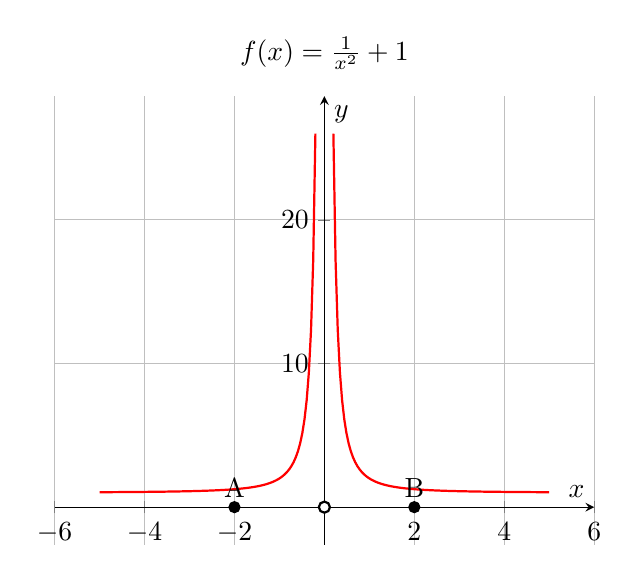
\begin{tikzpicture}
    \begin{axis}[
        title={$f(x) = \frac{1}{x^2} + 1$},
        axis lines = middle,
        grid = major,
        enlargelimits = true,
        xlabel={$x$},
        ylabel={$y$},
    ]
    
    % Función racional
    \addplot[domain=-5:-0.2, samples=100, thick, red] {((1)/(x^(2)))+1};
    \addplot[domain=0.2:5, samples=100, thick, red] {((1)/(x^(2)))+1};
    
    % Puntos marcados
    \addplot[only marks, mark=*, mark options={black}, nodes near coords={A}] coordinates {(-2,0)};
    \addplot[only marks, mark=*, mark options={black}, nodes near coords={B}] coordinates {(2,0)};
    \addplot[only marks, mark=*, mark options={white}, scale=1.5] coordinates {(0,0)};
    \addplot[only marks, mark=o, mark options={black}, scale=1.5, thick] coordinates {(0,0)};
    
    \end{axis}
\end{tikzpicture}
    \caption{Función racional decreciente y creciente antes y después de $c$ respectivamente.}
    \label{fig:racional1}
\end{figure}

\begin{figure}[H]
    \centering
    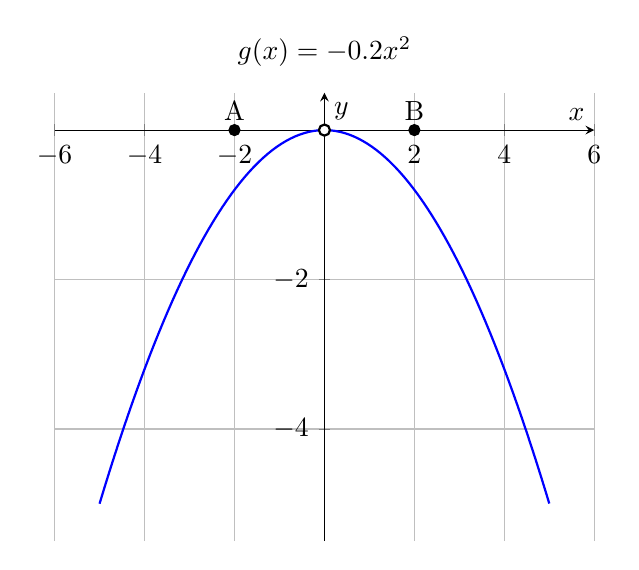
\begin{tikzpicture}
    \begin{axis}[
        title={$g(x) = -0.2x^2$},
        axis lines = middle,
        grid = major,
        enlargelimits = true,
        xlabel={$x$},
        ylabel={$y$},
    ]
    
    % Función cuadrática
    \addplot[domain=-5:5, samples=100, thick, blue] {-0.2*x^2};
    
    % Puntos marcados
    \addplot[only marks, mark=*, mark options={black}, nodes near coords={A}] coordinates {(-2,0)};
    \addplot[only marks, mark=*, mark options={black}, nodes near coords={B}] coordinates {(2,0)};
    \addplot[only marks, mark=*, mark options={white}, scale=1.5] coordinates {(0,0)};
    \addplot[only marks, mark=o, mark options={black}, scale=1.5, thick] coordinates {(0,0)};
    
    \end{axis}
\end{tikzpicture}
    \caption{Función cuadrática decreciente y creciente antes y después de $c$ respectivamente.}
    \label{fig:cuadratica1}
\end{figure}

\begin{itemize}
    \item Si \(f'(x)\) es negativa para todo \(x<c\), y \(f'(x)\) es positiva para todo \(x>c\), en el punto \(c\) hay un mínimo relativo de \(f\).
\end{itemize}

En este enunciado se podría aplicar la misma lógica que en el primero, pero abordaré en este el criterio de la segunda derivada. Una vez se hallan los puntos críticos igualando la primera derivada a cero, entonces se evavlúa la segunda derivada en dichos puntos y si $f''(x) > 0$ entonces la función es cóncava hacia arriba y si $f''(x) < 0$ entonces la función es cóncava hacia abajo.

Si la función es cóncava hacia arriba en un punto crítico, entonces es un mínimo relativo y si es cóncava hacia abajo, entonces es un máximo relativo. Sin embargo, en este caso no existen puntos críticos, ya que al igualar $f'(x) = 0$ no se obtiene ninguna solución. \textbf{Por lo tanto, el enunciado es falso}.

En las siguientes gráficas se puede apreciar lo anteriormente mencionado:

\begin{figure}[H]
    \centering
    \input{images/noRutinarios1,3.tex}
    \caption{Función racional creciente y decreciente antes y después de $c$ respectivamente.}
    \label{fig:racional2}
\end{figure}

\begin{figure}[H]
    \centering
    \input{images/noRutinarios1,4.tex}
    \caption{Función cuadrática creciente y decreciente antes y después de $c$ respectivamente.}
    \label{fig:cuadratica2}
\end{figure}